\chapter{Analysis and Benchmark\label{cha:chapter6}}

\section{Ground Truth}\label{sub:ground truth}
To assess the quality of the localization algorithm, the true position of the robot needed to be obtained in order to do the comparisons and benchmarks with the position calculated by the algorithm. The true position of the robot or the so called \textit{ground truth} can not be obtained from the robot itself, since it does not have built in \gls{GPS} or other position tracking sensors. Moreover, the accuracy within centimeters is required for this purpose. 

The approach adopted in this paper is SSL-Vision \cite{zickler2010ssl}, the vision system used in RoboCup Small Size League to obtain the position of the robots. SSL-Vision requires a camera mounted on the ceiling, and a marker with specific pattern on top of the robot. By detecting the marker and the field through the ceiling camera, the ground truth can be obtained. For NAO robot, since its head could be scanning left and right, the marker can not be directly attached on its head, otherwise the robot's orientation obtained is not correct. To counter this, a plastic support is printed using 3D printer. As illustrated by \autoref{fig:collage}, the support is worn by the robot from the back, and the marker is attached on the top of the support.

\begin{figure}[h!]
  \centering
  \includegraphics[width=.7\textwidth]{sslvision-collage.png}
  \caption{The 3D printed support and the pattern marker}
  \label{fig:collage}
\end{figure}

In the SSL-Vision software \cite{sslvision_yuan}, first set the field size, robot height, camera height and the corners of the field to calibrate the camera, so a point in the image plane can be mapped to the coordinate of the global frame. Then the colors in the field and the colors from the marker needed also to be calibrated. Shown in \autoref{fig:calibration} is the visualization result after calibration. When the marker is detected by SSL-Vision, the coordinate of the robot position in global frame will be broadcasted via network. The detected robot position is drawn in the field GUI in \autoref{fig:position}.\\

\begin{figure}[h!]
        \centering
        \begin{subfigure}[h]{0.59\textwidth}
                \includegraphics[width=\textwidth]{gt2.png}
                \caption{calibration result}
                \label{fig:calibration}
        \end{subfigure}%
        ~ %add desired spacing between images, e.g. ~, \quad, \qquad, \hfill etc.
          %(or a blank line to force the subfigure onto a new line)
        \begin{subfigure}[h]{0.41\textwidth}
                \includegraphics[width=\textwidth]{gt1crop.png}
                \caption{position in field}
                \label{fig:position}
        \end{subfigure}%
	\caption[SSL-Vision color and camera calibration result, and robot position result]{SSL-Vision color and camera calibration result (a), robot position result (b)}
	\label{fig:sslVision result}
\end{figure}


\noindent\textbf{Disadvantages of SSL-Vision}
\begin{itemize}
  \item The system highly depend on the light of the environment, once the surrounding light changes, the color metrics need to be recalibrated. 
  \item If the marker is printed using normal paper, it may cause reflection at certain angle from the view point of the camera, then the pattern can not be detected. For this reason, fuzzy materials are specially chosen to manually create the marker. 
  \item The system can not detect the pattern when the robot is fallen.
\end{itemize}

\section{Logging Perception and Ground Truth}
\label{sub:Logging Perception and Ground Truth}
For the purpose of debugging and benchmark, the robot can stores the perception as log for future replay. The log contains the necessary data needed to re-run the localization algorithm on another computer. Within the log, it includes vision results, odometry, \gls{IMU}, sonar data, time stamp, robot posture, etc. In order to benchmark the quality of the localization algorithm result, the ground truth data needed to be stored as well, and when the log is replayed, the ground truth data should be synchronized with the perception log. The solution for this is to store the broadcasted ground truth from SSL-Vision at the same of recording the perception, and the ground truth become part of the perception log. The replayed perception log with ground truth is already illustrated in \autoref{fig:landmarkRobotFrame}, in which the ground truth position indicated by red, calculated position in cyan, mirrored calculated position in pink.

%\begin{figure}[h!]
%  \centering
%  \includegraphics[width=.7\textwidth]{logagent.png}
%  \caption{perception log replayed with ground truth using particle filter localization (ground truth (red), calculated position (cyan), mirrored calculated position (pink))}
%  \label{fig:logagent}
%\end{figure}





\section{Code Optimization}
\label{sec:Optimization}
As illustrated in \autoref{sub:hardware}, the motherboard the robot equips is an embedded platform with only limited computation power. This requires the localization algorithms developed to be computational efficient in order to run in real time in \gls{SPL} game. In this section, the methods used to enhance the performance of the two localization algorithms, namely optimization based localization and multi-hypotheses Kalman filter localization, will be discussed.

By the intrinsic of the Rprop algorithm, optimization based localization imposes significant overhead in computation. On the one hand, it uses all the detected line points instead of line segments to calculate the measurement error, on the other hand, the optimization procedure takes several iterations to converge to the optimal result. Although the error function being used by Rprop has been implemented by an error look up table and an error gradient look up table, which saves the on-line computation time by pre-calculating the error and error gradient off-line, the computation time is still high. Initially the implementation is using the combination of python and Numpy. After optimizing the computation heavy part using Cython and reducing the number of optimization iterations, the computation speed has increased 84\%. However, with this speed up after optimization, it is still 5 times slower than the implementation of particle filter as illustrated in \autoref{tab:timecomp}, which is far from acceptable to run on the robot.

The major drawback pertains to the optimization based localization is that when the size of look up table is big, the requests to the look up table can often cause CPU cache miss if the data requested in memory is not contiguous. Since the line points in observation are often scattered over the field, and the look up table is constructed row by row along the field, a request to the look up table by these line points will often result in the penalty of cache miss. Moreover, two look up tables have to be requested and repeatedly for several iterations during the optimization step, which magnifies the overhead.

Taking the experience during implementing optimization based localization, the principle is to implement the computation heavy part using lower level programming language to gain performance and the other part in higher level language to have design flexibility.
For multi-hypotheses Kalman filter, the code pertaining to motion update and sensor update are implemented in \cpp. The other part of code regarding observation pre-processing and feature detection are implemented using the combination of python, Numpy and Cython. The interface between \cpp  code and python code is bridged by Cython. The performance of this design turns out to be satisfactory. As illustrated in \autoref{tab:timecomp}, it is 27.8\% faster than the speed of particle filter.

\section{Benchmarks}
\label{sec:Benchmark}
To benchmark the quality of localization algorithms, we use the same perception log with ground truth as the input for the different algorithms. The log is recorded when the robot is initially placed at the side of the field and walks into the goalie position. In the end, the robot is kidnapped to a position near the center circle \footnote{The kidnapping happens at around frame 3200 of the log, where a robot position ``jump'' is illustrated by the ground truth in \autoref{fig:benchmarkParticle}}. The quality of the localization algorithm is judged by the following criteria: 
\begin{enumerate}
  \item Initial global localization.
  \item Accuracy of robot position tracking.
  \item Recovery from tracking failure or kidnap.
  \item Efficiency of algorithm.
\end{enumerate}

Three localization algorithms are compared, namely, particle filter, optimization based localization, multi-hypotheses Kalman filter localization.

\subsection{Accuracy}
\label{sub:Accuracy}
The results of the localization with different algorithms are illustrated in 
\autoref{fig:benchmarkParticle}, \autoref{fig:benchmarkRprop} and \autoref{fig:benchmarkKalman}. In each figure, the first three sub-plots in the first row compare the localization result with the ground truth in $x$, $y$, $\theta$ dimension respectively. The forth sub-plot in the first row shows the moving trajectory of the robot for both calculated one and the ground truth. The second row of the sub-plots illustrate the error between the localization result and the ground truth.

\begin{figure}[h!]
\begin{center}
	%\includegraphics[width=\textwidth]{benchmark_trytogoalie_particle.png}
	\includegraphics[width=\textwidth]{benchmark_particle2.png}
\end{center}
\caption[Particle filter localization result compared with ground truth]{Particle filter localization result (blue) compared with ground truth (green)}
\label{fig:benchmarkParticle}
\end{figure}
%[('', '$E(e)$', '$\\delta(e)$'), ('$x$', 0.27794279267269395, 0.3492095080558556), ('$y$', 0.30230040992251561, 0.30502241418287196), ('$\\theta$', 0.32650508700053837, 0.38371622182735776), ('$d$', 0.44545705278503417, 0.43033905427307967)]

%paricle2
%[('', '$E(e)$', '$\\delta(e)$'), ('$x$', 0.55183942584722578, 0.59131139906929575), ('$y$', 0.42219593496159497, 0.40303767773039317), ('$\\theta$', 0.43895938658740813, 0.53193942003138717), ('$d$', 0.73857044381197312, 0.67035691932318597)]

\begin{figure}[h!]
\begin{center}
	\includegraphics[width=\textwidth]{benchmark_rprop.png}
\end{center}
\caption[Optimization based localization result compared with ground truth]{Optimization based localization result (blue) compared with ground truth (green)}
\label{fig:benchmarkRprop}
\end{figure}
%[('', '$E(e)$', '$\\delta(e)$'), ('$x$', 0.41285236480916204, 0.41123891005121205), ('$y$', 0.52180417053113137, 0.73911675845537628), ('$\\theta$', 0.52008518389747416, 0.70291834048810775), ('$d$', 0.7052172517778369, 0.81289994407479604)]

\begin{figure}[h!]
\begin{center}
	\includegraphics[width=\textwidth]{benchmark_trytogoalie_kalman.png}
\end{center}
\caption[Multi-hypotheses Kalman filter localization result compared with ground truth]{Multi-hypotheses Kalman filter localization result (blue) compared with ground truth (green)}
\label{fig:benchmarkKalman}
\end{figure}

%[('', '$E(e)$', '$\\delta(e)$'), ('$x$', 0.3114195849313835, 0.39319751044929591), ('$y$', 0.24561330872443066, 0.388151897485701), ('$\\theta$', 0.21089172180948793, 0.23866537659570336), ('$d$', 0.42042210261797613, 0.53462088312836409)]


In terms of localization accuracy, the average error and error deviation for each localization algorithm is shown in \autoref{tab:statistics}. From \autoref{tab:statistics}, we can see that multi-hypotheses Kalman filter out-performs the other localization algorithms in term of accuracy. By comparing \autoref{fig:benchmarkParticle} and \autoref{fig:benchmarkKalman}, another benefit of  Kalman filter based localization is that the trajectory of the position is more smooth than the one from particle filter.
\begin{table}[h!]
  \centering
  \caption{Accuracy comparison between different localization algorithms}
  \label{tab:statistics}
  \begin{adjustbox}{max width=\textwidth}
    \begin{tabular}{l|l|l|l|l|l|l|l|l}
      Average error  \& deviation & x (\SI{}{\meter})                   &  deviation     & y  (\SI{}{\meter})                   & deviation        & $\theta$  (\SI{}{\radian})            &deviation    & total error         &deviation           \\
      &                     & x (\SI{}{\meter})&                     &  y (\SI{}{\meter})&                     &  $\theta$ (\SI{}{\radian}) &                     & total error\\ \hline
      %Particle Filter                & 0.278 & 0.349 & 0.302 & 0.305 & 0.326 & 0.384 & 0.445 & 0.430   \\ \hline
      Particle filter                & 0.552& 0.591 & 0.422 & 0.403 & 0.439 & 0.532 & 0.739 & 0.670   \\ \hline
      Optimization based            & 0.413 & 0.411 & 0.522 & 0.739 & 0.520 & 0.703 & 0.705 & 0.813   \\ \hline
      Multi-hypotheses Kalman filter & 0.311 & 0.393 & 0.246 & 0.388 & 0.211 & 0.239 & 0.420 & 0.535  
    \end{tabular}
  \end{adjustbox}
\end{table}

\subsection{Functionality}
\label{sub:Functionality}

From the illustrations of the localization results, all the three localization algorithms solve the initial global localization problem and tracks the robot position after global localization. 

Concerning the ability to recover from kidnapped situation, only multi-hypotheses Kalman filter localization recovered the robot position at the end of the log. That is because the robot observed an ``X'' junction near the center circle, and resampling is triggered to recover the robot position. However, ``X'', ``T'' junction detection and resampling is only used in multi-hypotheses Kalman filter localization algorithm, not in particle filter and optimization based localization, therefore the other algorithm can not recover in this case. Particle filter localization is also capable to do resampling when ``L'' junction, penalty area or center circle are seen.

\subsection{Efficiency}
\label{sub:Efficiency}
Last but not least, the computation time for executing the log is measured for each algorithm to compare the efficiency.  The log is not executed on the robot but on a normal laptop, since the aim is to compare the efficiency between the algorithms. And in addition we know particle filter can be run seamlessly on the robot together with other necessary \gls{SPL} modules. So the log execution time of particle filter can be regarded as a base line for other algorithms. \autoref{tab:timecomp} depicts the execution time of the log for each localization algorithm\footnote{For detailed profiles of algorithm execution time, refer to \autoref{sec:profiles}}. Within \autoref{tab:timecomp}, multi-hypotheses Kalman filter localization out-performs the other localization algorithms in computation speed, and optimization based localization being the slowest.


% \begin{table}[h!]
% \centering
% \caption{Execution time comparison between different localization algorithms}
% \label{tab:timecomp}
%   \begin{adjustbox}{max width=\textwidth}
% \begin{tabular}{l|l|l|l}
%                                                 & Particle filter & Optimization Based & Multi-hypotheses Kalman filter \\ \hline
% Localization execution time (second) & 1.989           & 9.952              & 1.436                         
% \end{tabular}
%   \end{adjustbox}
% \end{table}


\begin{table}[h!]
\centering
\caption{Execution time comparison between different localization algorithms}
\label{tab:timecomp}
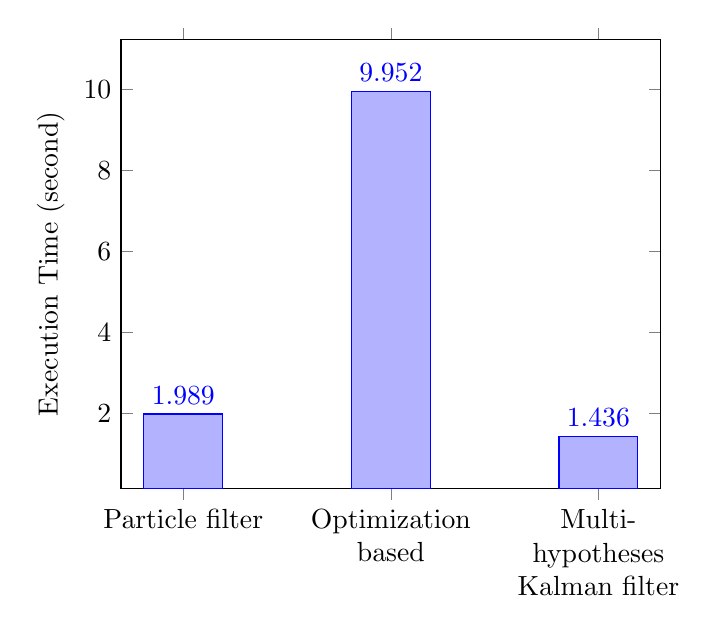
\begin{tikzpicture}
\begin{axis}[
    ybar,
    enlargelimits=0.15,
    legend style={at={(0.5,-0.15)},
      anchor=north,legend columns=-1},
    ylabel=Execution Time (second),
    symbolic x coords={Particle filter,Optimization based, Multi-hypotheses Kalman filter},
    xtick=data,
    bar width=1cm,
    nodes near coords,
    nodes near coords align={vertical},
    nodes near coords={\pgfmathprintnumber[fixed zerofill, precision=3]{\pgfplotspointmeta}},
    %x tick label style={rotate=-10,anchor=north},
    x tick label style={text width=2.2cm,align=center},
    ]
\addplot coordinates {(Particle filter,1.989) (Optimization based,9.952) (Multi-hypotheses Kalman filter, 1.436)};
%\legend{used,understood,not understood}
\end{axis}
\end{tikzpicture}
\end{table}
%Multi-hypotheses Kalman filter
%Optimization based localization turns out to be 5 times slower than particle filter.
